\documentclass[12pt,a4paper]{article}
\usepackage{amsmath,amscd,amsbsy,amssymb,latexsym,url,bm,amsthm}
\usepackage{epsfig,graphicx,subfigure}
\usepackage{float}
\usepackage{enumitem,balance}
\usepackage{wrapfig}
\usepackage{mathrsfs,euscript}
\usepackage[usenames]{xcolor}
\usepackage{hyperref}
\usepackage[vlined,ruled,linesnumbered]{algorithm2e}
\usepackage{array}
\hypersetup{colorlinks=true,linkcolor=black}

\newtheorem{theorem}{Theorem}
\newtheorem{lemma}[theorem]{Lemma}
\newtheorem{proposition}[theorem]{Proposition}
\newtheorem{corollary}[theorem]{Corollary}
\newtheorem{exercise}{Exercise}
\newtheorem*{solution}{Solution}
\newtheorem{definition}{Definition}
\theoremstyle{definition}

\renewcommand{\thefootnote}{\fnsymbol{footnote}}

\newcommand{\postscript}[2]
 {\setlength{\epsfxsize}{#2\hsize}
  \centerline{\epsfbox{#1}}}

\renewcommand{\baselinestretch}{1.0}

\setlength{\oddsidemargin}{-0.365in}
\setlength{\evensidemargin}{-0.365in}
\setlength{\topmargin}{-0.3in}
\setlength{\headheight}{0in}
\setlength{\headsep}{0in}
\setlength{\textheight}{10.1in}
\setlength{\textwidth}{7in}
\makeatletter \renewenvironment{proof}[1][Proof] {\par\pushQED{\qed}\normalfont\topsep6\p@\@plus6\p@\relax\trivlist\item[\hskip\labelsep\bfseries#1\@addpunct{.}]\ignorespaces}{\popQED\endtrivlist\@endpefalse} \makeatother
\makeatletter
\renewenvironment{solution}[1][Solution] {\par\pushQED{\qed}\normalfont\topsep6\p@\@plus6\p@\relax\trivlist\item[\hskip\labelsep\bfseries#1\@addpunct{.}]\ignorespaces}{\popQED\endtrivlist\@endpefalse} \makeatother

\begin{document}
\noindent

%========================================================================
\noindent\framebox[\linewidth]{\shortstack[c]{
\Large{\textbf{Lab11-NP Reduction}}\vspace{1mm}\\
CS214-Algorithm and Complexity, Xiaofeng Gao \& Lei Wang, Spring 2021.}}
\begin{center}
\footnotesize{\color{red}$*$ If there is any problem, please contact TA Yihao Xie. }

\footnotesize{\color{blue}$*$ Name:Yanjie Ze \quad Student ID: 519021910706 \quad Email: zeyanjie@sjtu.edu.cn}
\end{center}

\begin{enumerate}
    \item We are feeling experimental and want to create a new dish. There are various ingredients we can choose from and we'd like to use as many of them as possible, but some ingredients don't go well with others. If there are $n$ possible ingredients (numbered 1 to $n$), we write down an $n\cdot n$ matrix giving the discord between any pair of ingredients. This discord is a real number between 0.0 and 1.0, where 0.0 means "they go together perfectly" and 1.0 means "they really don't go together." Here's an example matrix when there are five possible ingredients.
    \begin{center}
        \begin{tabular}{|c|ccccc|}
        \hline
             & 1  & 2 & 3 & 4 & 5\\
        \hline
            1 & 0.0 & 0.4 & 0.2 & 0.9 & 1.0\\
            2 & 0.4 & 0.0 & 0.1 & 1.0 & 0.2\\
            3 & 0.2 & 0.1 & 0.0 & 0.8 & 0.5\\
            4 & 0.9 & 1.0 & 0.8 & 0.0 & 0.2\\
            5 & 1.0 & 0.2 & 0.5 & 0.2 & 0.0\\
        \hline
        \end{tabular}
    \end{center}
    In this case, ingredients 2 and 3 go together pretty well whereas 1 and 5 clash badly. Notice that this matrix is necessarily symmetric; and that the diagonal entries are always 0.0. Any set of ingredients incurs a penalty which is the sum of all discord values between pairs of ingredients. For instance, the set of ingredients $(1,3,5)$ incurs a penalty of $0.2+1.0+0.5 = 1.7$. We define the \textsc{Experimental Cuisine} as follows:

        Given $n$ ingredients to choose from, the $n\times n$ discord matrix and integer $k$ and a number $p$,  decide whether there exists a collection of at least $k$ ingredients that has a penalty $\leqslant p$

    Prove that $\textsc{3-SAT}\leq_p\textsc{Experimental Cuisine}$
    
    \begin{proof}
    ~\\
   \textbf{Basic idea:} By proving that INDEPENDENT-SET $\leq_p$ EXPERIMENTAL CUISINE, we prove that 3-SAT $\leq$ EXPERIMENTAL CUISINE.
   
   ~\\
   We construct a graph $G$. Each vertex $v$ in $G$ represents an ingredient. 
   
   For the edges of $G$:
   \begin{itemize}
       \item 
   If the discord between the ingredient $i$ and the ingredient $j$ is 0, the edge $e(i,j)$ between the vertex $v_i$ and the vertex $v_j$ does not exist.
  \item 
   If the discord between the ingredient $i$ and the ingredient $j$ is not 0, the edge $e(i,j)$ between the vertex $v_i$ and the vertex $v_j$ exists.
       \end{itemize}
       
       \textbf{Claim:} \textit{there exists an independent set of size at least k iff there exists an experimental cuisine collection of at least $k$ with a penalty=0.}
       
       $\Rightarrow$
      If in $G$ there exists an independent set of size at least $k$, then there must exists an experimental cuisine collection of at least $k$ with a penalty $p=0$. Since each vertex in $G$ represents an ingredient, we use the set consisting of corresponding ingredients of the vertices in the independent set as the cuisine.
    
      $\Leftarrow$ If there exists a cuisine collection of size at least $k$ with a penalty $p=0$, we can use the corresponding vertices of the ingredients to construct the independent set, with size of at least $k$.
      
      Therefore, we prove that INDEPENDENT-SET $\leq_p$ EXPERIMENTAL CUISINE.
      
      ~\\
      By 3-SAT $\leq_p$ INDEPENDENT-SET  and INDEPENDENT-SET $\leq_p$ EXPERIMENTAL CUISINE,  we have:\begin{center}
      3-SAT  $\leq_p$ EXPERIMENTAL\ CUISINE. 
          \end{center} 
    \end{proof}
    \item An induced subgraph $G'=(V',E')$ of a graph $G=(V,E)$ is a graph that satisfies $V'\subseteq V$ and $E' =\{(u,v)\in E| u,v\in V'\}$. Given two graphs $G_1=(V_1,E_1)$ and $G_2=(V_2,E_2)$ and an integer $b$, we need to decide whether $G_1$ and $G_2$ have a common induced subgraph $G_c$ with at least $b$ nodes. This problem is called \textsc{Maximum Common Subgraph} (MCS). Prove that MCS is NP-complete. (Hint: reduce from \textsc{INDEPENDENT-SET})
\begin{solution}
    ~\\
    We construct two graphs $G_1=(V,E)$ and $G_2=(V,\emptyset)$.
    
    We prove that given a graph $G_1$, $G_1$ has the independent set of size at least $b$ if and only if $G_1$ and $G_2$ have a common induced subgraph $G_c$ with at least $b$ nodes.
    
    \textbf{Claim:} $G_1$ has the independent set of size at least $b$ iff $G_1$ and $G_2$ have a common induced subgraph $G_c$ with at least $b$ nodes.
    
    
    \textbf{Proof:}
    ~\\
    $\Rightarrow$ $G_1$ has the independent set $V_{ind}$ of size at least $b$. Then the maximum common subgraph $G_c$ of $G_1$ and $G_2$ has exactly the same vertices as $V_{ind}$, and no edges are in $G_c$. Therefore, $G_c$ has at least $b$ nodes.
    
    $\Leftarrow$ The maximum subgraph $G_c$ of $G_1$ and $G_2$ has at least $b$ nodes. Then the vertices of $G_c$ are the same as the vertices in the independent set $V_{ind}$. Therefore, $V_{ind}$ has the size of at least $b$.
    

Therefore, INDEPENDENT-SET $\leq_p$ MCS, and MSC is \textbf{NP-complete}.
    
\end{solution}
    \item Let us define the $k$-spanning tree as a spanning tree in which each node has a degree $\leqslant k$. Given a graph $G= (V,E)$ and a positive integer $k$, we need to decide whether there exists a $k$-spanning tree in $G$. Prove that this problem is NP-complete. (Hint: reduce from \textsc{HAMILTONIAN-CYCLE})
    \begin{solution}
    ~\\
        \textbf{Basic idea}: We prove in the following order: 
        \begin{enumerate}
            \item HAMILTONIAN-CYCLE $\leq_p$ HAMILTONIAN-PATH
            \item HAMILTONIAN-PATH $\leq_p$ K-SPANNING TREE
            \item HAMILTONIAN-CYCLE $\leq_p$ K-SPANNING TREE
        \end{enumerate}

\textbf{Proof}:
\begin{enumerate}
    \item HAMILTONIAN-CYCLE $\leq_p$ HAMILTONIAN-PATH
    
    Given a graph $G=(V,E)$, we construct a new graph $G'$ such that $G$ contains a HAMILTONIAN-CYCLE if and only if $G'$ contains a HAMILTONIAN-PATH.
    
    Construct $G'$:
    \begin{enumerate}
    \item Copy all the edges and all the vertices of $G$ in $G'$, as shown in Fig.~\ref{fig3}.
    \begin{figure}[H]
        \centering
        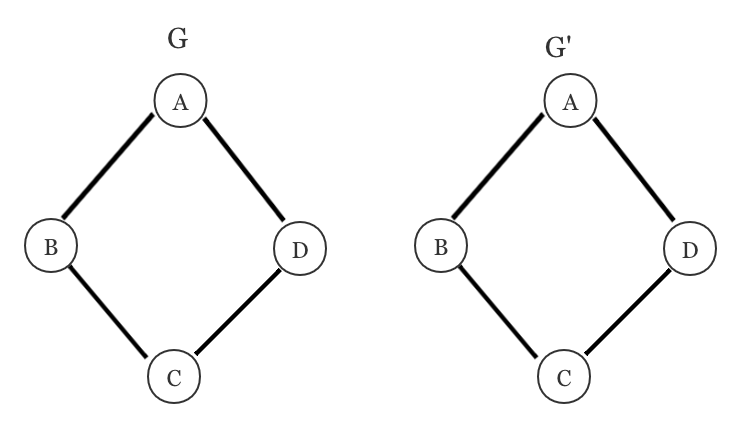
\includegraphics[width=8cm]{3.png}
        \caption{Construct $G'$, step 1}
        \label{fig3}
    \end{figure}
        \item Select a random vertex $v$ in $G'$. Create another new vertex named $v'$ and connect $v'$ to all the vertices that $v$ is connected to, as shown in Fig.~\ref{fig1}.
                \begin{figure}[H]
            \centering
         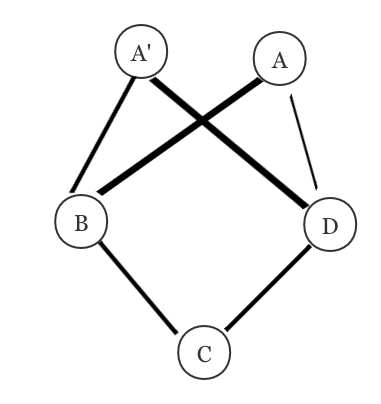
\includegraphics[width=4cm]{1.png}
            \caption{Construct $G'$, step 2}
          \label{fig1}
        \end{figure}
        \item Add two more vertices as the start point and the end point. Connect the start point with $v'$ and the end point with $v$, as shown in Fig.~\ref{fig2}.
        \begin{figure}[H]
            \centering
            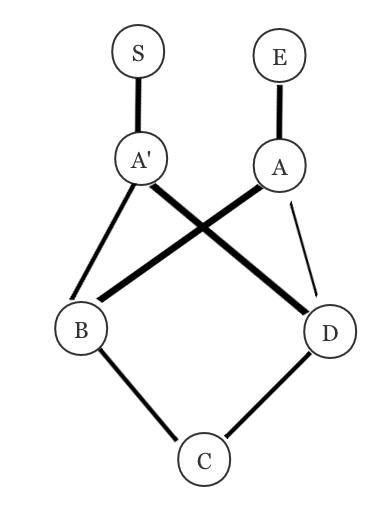
\includegraphics[width=4cm]{2.png}
            \caption{Construct $G'$, step 3}
            \label{fig2}
        \end{figure}
    \end{enumerate}
    
    If $G$ contains a HAMILTONIAN-CYCLE, there exists a HAMILTONIAN-PATH in $G'$, starting from the start point and ending at the end point.
    
    For the example we construct, the HAMILTONIAN-CYCLE in $G$ is $$\{(A,B),(B,C),(C,D),(D,A)\}$$ Then in $G'$, the HAMILTONIAN-PATH is $$\{(S,A'),(A',B),(B,C),(C,D),(D,A),(A,E)\}$$
    
    If $G'$ contains a HAMILTONIAN-PATH, we can transform this path in $G'$ into the HAMILTONIAN-CYCLE in $G$. This is because the HAMILTONIAN-PATH in $G'$ must pass the start point and the end point. We delete them  and make $v'$ back to $v$, which will transform the HAMILTONIAN-PATH in $G'$ into the HAMILTONIAN-CYCLE in $G$.
    
    For this example, in $G'$, the HAMILTONIAN-PATH is $$\{(S,A'),(A',B),(B,C),(C,D),(D,A),(A,E)\}$$
    Delete $S$, $E$, $A'$ and transform $(A',B)$ into $(A,B)$. Then $G'$ becomes $G$ and HAMILTONIAN-PATH becomes HAMILTONIAN-CYCLE:
     $$\{(A,B),(B,C),(C,D),(D,A)\}$$
     
     Thus, we prove that HAMILTONIAN-CYCLE $\leq_p$ HAMILTONIAN-PATH.
     
     \item 
     HAMILTONIAN-PATH $\leq_p$ K-SPANNING TREE
     
     Given a graph $G$, $G$ contains a HAMILTONIAN-PATH iff $G$ contains a k-spanning tree ,$k=2$.
     
     This is easy to prove, since a HAMILTONIAN-PATH is exactly a special case of the k-spanning tree. When $k=2$, the nodes either has the degree 1 or degree 2, which means this tree is also a path. 
     
     Therefore,  HAMILTONIAN-PATH $\leq_p$ K-SPANNING TREE.
     
     \item HAMILTONIAN-CYCLE $\leq_p$ K-SPANNING TREE
     
     From (a) and (b) we know that:
     HAMILTONIAN-CYCLE $\leq_p$ HAMILTONIAN-PATH, 
    HAMILTONIAN-PATH $\leq_p$ K-SPANNING TREE
    
    Therefore, HAMILTONIAN-CYCLE $\leq_p$ K-SPANNING TREE. 
    ~\\
    
    Since HAMILTONIAN-CYCLE is NP-Complete, K-SPANNING TREE is also NP-Complete.
    
    
\end{enumerate}

    \end{solution}
    \item We define the decision problem of \textsc{Knapsack Problem} as follows:
    
        Given $n$ indivisible objects, each with a weight of $w_i>0$ kilograms and a value $v_i>0$, a knapsack with capacity of $W$ kilograms and a number $k$, decide whether there is a collection of objects that can be put into the knapsack with a total value $V\geqslant k$.
        
    Prove that \textsc{Knapsack Problem} is NP-complete.
    
\end{enumerate}

\begin{solution}
~\\
\par
    \textbf{Basic idea}: We can prove that SUBSET-SUM $\leq_p$ KNAPSACK PROBLEM.
    
    
    \textbf{SUBSET-SUM}: Given a set $S$ of non-negative integers ,$S=\{s_1,s_2,...,s_n\}$, does there exist a subset of $S$ with the sum of its elements equal to $T$?
    
    \textbf{Reduction:}
    Given a set $S=\{s_1,s_2,...,s_n\}$ consisting of non-negative numbers, We construct a knapsack with capacity $W=T$, and set the value threshold $k=T$. 
    
    We set $n$ indivisible objects, each with a weight of $w_i=s_i$.
    
    \textbf{Claim:}
    The set $S$ has a subset with the sum of elements equal to $T$ iff there exists a collection of objects that can be put into the knapsack with a total value $V=T$.
    
    $\Rightarrow$ If the set $S$ has a subset with the sum of elements equal to $T$, the element of this subset will correspond to one object, $w_i=s_i$. Then we place these corresponding objects in the knapsack, which will have a total value of $T$.
    
    $\Leftarrow$ If there exists a collection of objects that can be put into the knapsack with a total value $V=T$, we construct the subset $S'$ of $S$. The elements of $S'$ are the  elements corresponding to the objects in the knapsack, $s_i=w_i$. Therefore, the sum of elements in $S'$ is equal to $T$.
    
    Thus, SUBSET-SUM $\leq_p$ KNAPSACK PROBLEM.
    ~\\
    
    Since SUBSET-SUM is NP-Complete, KNAPSACK PROBLEM is also NP-Complete.
    
    
    
    
    
    
    
    
\end{solution}
\textbf{Remark:} Please include your .pdf, .tex files for uploading with standard file names.
\newpage


%========================================================================
\end{document}